%% This LaTeX-file was created by Maarten van Leunen

%% Do not edit this file unless you know what you are doing.
\documentclass{article}
\usepackage{times}
\usepackage{graphics}

\begin{document}
\author{Maarten van Leunen}
\title{MMUD\\Maarten's Mud}
\maketitle
\tableofcontents
\listoffigures
\listoftables
\newpage

\subsection{Legal Notice}
\begin{verbatim}
/*-------------------------------------------------------------------------
Maarten's Mud, WWW-based MUD using MYSQL
Copyright (C) 1998  Maarten van Leunen

This program is free software; you can redistribute it and/or
modify it under the terms of the GNU General Public License
as published by the Free Software Foundation; either version 2
of the License, or (at your option) any later version.

This program is distributed in the hope that it will be useful,
but WITHOUT ANY WARRANTY; without even the implied warranty of
MERCHANTABILITY or FITNESS FOR A PARTICULAR PURPOSE.  See the
GNU General Public License for more details.

You should have received a copy of the GNU General Public License
along with this program; if not, write to the Free Software
Foundation, Inc., 59 Temple Place - Suite 330, Boston, MA  02111-1307, USA.

Maarten van Leunen
Driek van Erpstraat 9
5341 AK Oss
Nederland
Europe
maarten_l@yahoo.com
-------------------------------------------------------------------------*/
\end{verbatim}

\subsection{Acknowledgements}
I'd like to thank all the people that have been a support to me for so long
over the years. The Land of Karchan has had it's ups and downs over the
years as some of you might know, but now the source code is available with
which the Land of Karchan was created, and everyone who is familiar with
Linux can join and make their own.

I'd like to thank some of the people especially who helped me to build the
source code and were actually invaluable to me by giving practical advice
concerning source code. In no particular order they are Edwin Mons (edwinm), Mathijs
Brands (shrike), Joop Carels (zombie), Sven Berkens (sven), George Schroder
(frodpo). I also like to thank Steffan O'Sulivan for his excellent booklet
about "FUDGE" which helped me out a lot. I also like to thank Samual Jackson
Games for providing "GURPS" from which I learned a lot. I also like to thank the people
without whom this might never have come off the ground, the people of the
Open Source Movement, who have liberally provided me with the tools I needed
to make the Land of Karchan a reality.

\subsection{About the Author}
Well, let me introduce myself. I am Maarten van Leunen, currently living in
Oss, the Netherlands, Europe. Basically, when I entered College I for the
first time got into contact with Unix like Operating Systems, not by
studying, but by joining in the local InternetUsersAssociation Interlink. I aquired lots
of experience and knowledge there.

The first step towards creating a mud, ofcourse, is playing one. I happened
to frequent some time on Angalon, however, in time one has ambitions to
create one's own mud. At the same time, I was working on my first Homepage,
my first Guestbook. And when surfing I found out about a Mud consisting
entirely of links on the World Wide Web. I thought the idea was nifty, and
tried my hand at it. Then the idea crossed my mind to attempt to integrate
the experience I got from creating my Guestbook and my Homepage with the
experience of creating a Linked Mud. Apparently it has come this far, and
there is no end in sight just yet.

\newpage
\section{Installation}
\subsection{Root Priviledges}
It's a really bad idea to have this mud running under Root privileges. It's
a security issue. In stead, I suggest that you create a new user on your
server called "mmud". (or something else, in which case you need to make
some changes to the source code)

It's a mistake to run any kind of CGIbinary which is accessible from the
outside setuid root. It gives crackers the opportunity to enter your system
using this CGI.

{\par\centering \resizebox*{1\textwidth}{!}{\rotatebox{270}{\includegraphics{sourcecode.ps}}} \par}

\subsection{Password Authorisation}
There are currently two passwords. The first password (the real one) is used
only once, during logging into the game. It is the password that is
remembered by the user. The second password is called the 'SessionPassword'
and is generated by the server upon logging into the game, and is used
instead of the normal password during gameplay. This in order to prevent
having to submit a password accross the internet connection every time.

This allows for a significant improvement in security. See also the part
about cookies, for a diagram of the current authorisation procedure.

\subsection{Cookies}
Cookies play an important part of the game, as they provide a mechanism for
checking if a certain person is busy multiplaying, i.e. he/she is using two
different player characters on the same computer/account or he/she is using
two the same player characters on two different computers.

This also relates to password authorisation. I will attempt to explain the
process. Upon logging into the game, first is checked if a cookie already
exists. If the person is attempting to log on and there is a cookie, then a
warning of multiplaying is displayed. If there is a cookie, and the person
is attempting to relogon as the character that also contains the same
cookie, everything works fine.

During gameplay, the cookie is compared to the SessionPassword in the
database every time. 

{\par\centering
\resizebox*{1\textwidth}{!}{\rotatebox{270}{\includegraphics{cookie.ps}}} \par}

\newpage
\section{Playing the game}
\subsection{Character Defaults}
The five main attributes of your character are:
\begin{itemize}
\item Strength
\newline
You can carry more if you are stronger.
\item Intelligence (mental skills)
\newline

\item Dexterity (physical skills)
\newline
Dexterity is a measurement of agility and coordination. Basically it says
how clumsy you are (or not).
\item Constitution
\item Wisdom
\end{itemize}

The five main attributes of an Elf are:
\begin{itemize}
\item Strength 2
\item Intelligence (mental skills) 2
\item Dexterity (physical skills) 1
\item Constitution 2
\item Wisdom 2
\end{itemize}

The five main attributes of an Dwarf are:
\begin{itemize}
\item Strength 2
\item Intelligence (mental skills) 1
\item Dexterity (physical skills) 2
\item Constitution 2
\item Wisdom 0
\end{itemize}

The five main attributes of a standard Human are:
\begin{itemize}
\item Strength 1
\item Intelligence (mental skills) 1
\item Dexterity (physical skills) 1
\item Constitution 1
\item Wisdom 1
\end{itemize}

The five main attributes of a Faery are:
\begin{itemize}
\item Strength 0
\item Intelligence (mental skills) 2
\item Dexterity (physical skills) 1
\item Constitution 1
\item Wisdom 2
\end{itemize}

\subsection{Weight and Encumberance}
The amount of stuff you are carrying and the amount of strength you have
determines how much of your movement is spent on each move.

\begin{itemize}
\item weight < 500 + 50*Strength => no penalty
\item weight < 1000 + 50*Strength => move penalty of 10
\item weight < 1500 + 50*Strength => move penalty of 20
\item weight < 2000 + 50*Strength => move penalty of 30
\item weight < 2500 + 50*Strength => move penalty of 40
\item weight < 3000 + 50*Strength => move penalty of 50
\item weight >= 3000 + 50*Strength => UNABLE TO MOVE
\end{itemize}

So, to summarize. If you carry too much, you cannot move. The more you
carry, the more you get exhausted (i.e. lose movement points). Once you are
exhausted you cannot move. You recover over time, but it takes some time to
recover fully.
The stronger you are, the more you can carry and the less movement points it
takes for you to move.

\subsection{Skills}

Skills are defined as Items in this game. It is for example possible to own
an item called "\emph{Swordplay}". The Skilllevel inherent to the item is
stored in "skillevel". The skilllevel is a minimum of 0 and a maximum of 18.
If you have not "learned" the skill, the item does not exist.

A skill is relative to one of the five main attributes of your character.
The five main attributes of your character are:
\begin{itemize}
\item Strength
\item Intelligence (mental skills)
\item Dexterity (physical skills)
\item Constitution
\item Wisdom
\end{itemize}

If your skill level reaches beyond a certain level, as to be successfull
without really trying, the skill (in case for example with magic skills)
must be removed or automatically changed onto a higher skill. For example a
magic skill cast "\emph{burning candle}" should automatically revert to the
beginning level of "\emph{small fireball}" possibly converging all the way
to "\emph{firestorm}".

\subsection{Success Rolls}
A "success roll" is a die roll made when you need to "test" one of your
skills or abilities.. You roll against something, for instance an ability with an
Skill. This game predominately uses rolls against skills in order to see if
they will succeed or not. If your roll is less than or equal to the skill or
ability you are testing, you succeeded. Otherwise, you failed. Thus, the
higher the stat you are rolling against, the easier it is to make the roll.

For instance, if you have a skill "Swordplay", with "skillevel" 10, you roll
three dice. If the number of eyes is below or equal to 10, you succeed
otherwise you fail. A roll of 17 or 18 is an automatic and possibly
spectacular failure to practise the skill.

Ofcourse, you only need a "successroll" if you have a sword in your hand and
a skill "Swordplay". Otherwise the successroll is irrelevant. In the case
where a person is not holding anything in his hands, success will be
dependent on your skill at "unarmed combat".

\paragraph{Critical Success and Critical Failure}
There is such a thing as critical success if you (the computer) rolls the
dice and the outcome is either 3 or 4. This constitutes a critical success
with exceptional results if possible. A critical success has no chance of a
defense, all your hits strike home at your opponent.

There is such a thing as a critical failure if you (the computer) rolls the
dice and the outcome is 18. This constitutes a critical failure with
inordinately bad results.

\subsection{Reaction Rolls}
Not implemented yet. Perhaps not necessary.

\subsection{Defense Rolls}
Your foes defence equals \emph{passive} and \emph{active} defenses.
Passive defense is \emph{armour} and \emph{shields}. Active defense are skills
like \emph{dodge}, \emph{block}, \emph{parry}.

If the defense is successfull, no damage is done, and no damage roll is
executed.

\subsection{Damage Rolls}
A damage rolls is done in order to see how much damage you to do to your
opponent. A few things can effect the amount of damage you do, for instance:

\begin{itemize}
\item armour
\item weapon
\end{itemize}

\subsection{Learning and Improving Your Character}
Learning and Improving your character can be done by a lot of different
ways.

\begin{itemize}
\item killing bots (NPC - Non Player Characters)
\item solving quests
\end{itemize}

The two items explained above will create experience points. When enough
experience points have been gathered, you will "\emph{level}". Levelling will
provide you with two extra practise sessions and one extra training sessions
with which to improve your character further. Please note the next Paragraph
concerning practise and training.

\paragraph{Experience gained from NPCs}

The experience you gain from an NPC is computed in the following fashion:

\paragraph{Practise and Training}

Improving your character is done by learning a skill first, and then
improving upon it.

You can learn Skills by using the "\emph{practises}" which you have gained
when levelling. Every time you level, you gain 1 practise. That can be spent
on learning a certain skill.

You can improve Skills by using the "\emph{practises}" which you have gained
when levelling. Every time you level, you gain 1 practise. That can be spent
on a certain skill to up it one point.

You can improve your standard attributes by using the "\emph{training}"
points you got when you levelled. It can be used to gain a point in one of
the 5 attributes:
\begin{itemize}
\item Strength
\item Intelligence (mental skills)
\item Dexterity (physical skills)
\item Constitution
\item Wisdom
\end{itemize}

\section{Special Rooms}
\subsection{Moneychanger Office}
The money changers office has a special meaning. It can translate your coins
to another currency value (gold, copper, or silver) and you can open and
close and mutate an account there. For the most part it works just like a
bank.

To explain how the translation of coins work, we have to realize that, if we
use the copper coins as common denominator, the gold coins are worth 100
copper coins and the silver coins are worth 10 copper coins. A simple   
calculation does suffice to make converting values possible.

To explain how the bank principle works. If you open an account three items
in the tmp\_itemtable are created. Item 36 is copper coins, search=you,
room=-1 and the rest is empty. The same goes for Item 37 (silver) and item
38 (gold). The "amount" field takes care of the amount of gold silver or  
copper coins you have in your account. Withdraw and deposit simply mutate 
the gold, silver, copper fields in your character sheet as well as the    
amount in the different tmp\_itemtable items.

\section{Special Items}
\subsection{Containers}
There are special items in the game that can be called containers. The
definition of container being in this case: an item that can contain other
items. A container can also be empty.

The way it is implemented now is that there are two commands called 'put'
and 'retrieve' for manipulating items that are in containers or should be in
containers.

The way it is stored in the database is by means of a secondary table that
contains all the items that are contained in containers. The tmp\_itemtable
is the table that contains the containers. The following four combinations
can be determined:
\begin{itemize}
\item tmp\_itemtable.containerid=0 and items.container=0, this is the normal
situation, this means the item is not a container.
\item tmp\_itemtable.containerid=0 and items.container<>0, this is
acceptable, it means that the item can be a container, but right now doesn't
contain anything, i.e. is empty.
\item tmp\_itemtable.containerid<>0 and items.container<>0, this is the big
one, it means that the item is a container and that there are actually items
contained in this container.
\item tmp\_itemtable.containerid<>0 and items.container=0, this is an
illegal situation that should not occur.
\end{itemize}

The following two diagrams depict the algorithm used for retrieving an item
from a container and for putting an item into a container.

{\par\centering
\resizebox*{1\textwidth}{!}{\rotatebox{0}{\includegraphics{containers.ps}}} \par}
{\par\centering
\resizebox*{1\textwidth}{!}{\rotatebox{0}{\includegraphics{containers2.ps}}} \par}


\section{Combat}
\subsection{Who is fighting who?}
The only way to determine wether or not a person is fighting another person
and wether or not it is necessary to compute hits and start whacking each
other depends on a number of settings, written down here.

First of all, we will proceed from the assumption that character X is
fighting character Y. We now have to determine if this fight is actually
legal. The following constraints apply:
\begin{itemize}
\item ExistUser(X) == true (User X is active in the game)
\item ExistUser(Y) == true (User Y is active in the game)
\item X.sleep == false (User X is not asleep)
\item Y.sleep == false (User Y is not asleep)
\item X.room == Y.room (User X and Y are in the same room together)
\item Y.god != 2 (User Y is not a non-killable bot)
\item X.fightable == true (User X may fight people)
\item Y.fightable == true (User Y may be fought against)
\item X.fightingwho == Y.name (User X is definitely trying to fight User Y)
\end{itemize}
This part translates into the following SQL statement that has been used in
the "rolls.c" file:
\begin{itemize}
\item select X.*, Y.* from tmp\_usertable as X, tmp\_usertable as Y where
X.fightingwho = Y.name and
X.sleep = 0 and
Y.sleep = 0 and
X.room = Y.room and
Y.god != 2 and
X.fightable = 1 and
Y.fightable = 1;
\end{itemize}

{\par\centering
\resizebox*{1\textwidth}{!}{\rotatebox{270}{\includegraphics{compute_hit.ps}}} \par}

\subsection{Defense}
Every item that you use in combat has both a passive defense and an active
defense. The passive defense is the defence the item gives you without you
having to do anything (for example, making you hard to hit), the active
defense is when you actively do something with the item (like parry).

Melee:	any combat that involves striking the opponent with a fist or
hand-held weapon. Any attack from further away is a Ranged attack.
Alternating combat turns.

Combat Round: an indeterminate length of time set by the GM - around three
seconds seems reasonable to some people, while that seems grossly short or
absurdly long to others. A given GM's combat round may vary in length,
depending on the situation. Generally, when each character involved has made
an action, a given round is over.

Offensive damage factors: those which contribute to damaging an opponent
Strength (is using a Strength-driven weapon) Scale and deadliness of
weapon.

Defensive damage factors: those which contribute to reducting the severity
of a received blow: Scale, armor, and possibly Damage Capacity.

Total damage factor (or simply damage factor): the attacker's offensive
damage factor minus the defender's defensive damage factor.

\subsection{Illness, injury and Fatigue}

\subsection{Magic}

\section{Generating Miscellaneous Files}
\subsection{Maps}
Maps will be created using Gimp. The text contained on the map is "times" and the size = 12.

\subsection{Banners}
Banners for use on other websites will be created using Gimp. 
Lucidux serif (36)



\subsection{Documentation}
All documentation of the game will be done in the format of "Latex" (.tex)
Diagrams will be written with XFIG and included using the .pdf and .ps format.

In order to generate the different formats for viewing of the documentation,
the following commands are available: generate dvi (latex mmud.tex),
generate pdf (pdflatex mmud.tex), generate ps (pdf2ps mmud.pdf). This would
generate four different format files: .tex, .dvi, .pdf, .ps .

\section{The Parser}
\subsection{Introduction}
The Parser is a part of the program that is able to download source code
from the database and interpret the commands and execute them immediately.
The setup is quite simple and not meant to do anything drastic, but suffices
in most cases to execute special actions in rooms or for persons.

What follows first is a thorough explanation/reference guide for this new
scripting language. I am sorry to say that this is a quick hack, and
therefore does not work according to standard programming or scripting
languages that are currently in use for muds.

All source code is retrieved from the database. In order to be able to do
that the database has to have a number of tables. See for more information
the section on databasetables.

\paragraph{Databasetables}
The following tables are available:

\subparagraph{commands}commands contain the commands that a user is allowed
to enter, with references to the method that needs to be executed upon
entering one of these commands.
\subparagraph{methods}contains the id,name and sourcecode of a method to be
executed.
\subparagraph{events}contains events that run source code in the methods
table at specific times
\subparagraph{attributes}can contain 'special' attributes for characters,items,
rooms or even the game

Commands have a number of requirements before they can be executed, I will
attempt to name them here:
\begin{itemize}
\item the command entered by the user is compared to the value in 
\item callable needs to be unequal to 0, otherwise the command is disabled.
\item room needs to be either the same room the user is in or 0. If the room
in the commands table equals zero, this means that the command can be
executed from any other room.
\item the method\_name refers to the method in the methods table to be
executed
\end{itemize}

Hint: it is much easier to simply use an update statement as described below
instead of putting the source code into the insert statement as well.

Examples:
\begin{itemize}
\item insert into commands values(2, "yawn", 1, "yawn", "yawn", "", 0)
\item insert into methods values(2,"yawn","")
\item update methods set src = "say(\"You yawn.<BR>\")
sayeveryone(\"%me yawns.<BR>\")
showstandard
return
" where id = 2;

See below for more information concerning the events table and the attributes
table.

\end{itemize}

\subsection{Reference Guide}

\paragraph{General Principles}
The programming language is quite simply setup and therefore is not that
powerful. Here is some general stuff that should be applicable anywhere.

\begin{itemize}
\item if the parser does not recognize the first few syllables in the string, it
is discarded
\item following the rule above it is quite simple to add comments, but the
guideline is to make comments by prefixing them with the
\# (hash) sign.
\item indenting your code is fine, the interpreter has no problem with this, as
long as you use the tab to do this. All tabs at the beginning of each line
are discarded. (DO NOT USE SPACES!) I urge you to make good use of
indenting, it clarifies code immensely.
\item sometimes you would wish to wrap one command over multiple lines. This is
possible by appending a \ (slash) at the end of the line.
\item a new command has to start at a new line
\item for god's sake, be careful with SQL statements. The QUOTES are totally
screwed up. Meaning that you have to use double quotes in an sql
statement to make it absolutely clear that you want to store a QUOTE in a
text field instead of terminating a string. See also the little note at the
beginning of the examples.
\end{itemize}

\paragraph{Parameters}

What
I am talking about is substituting environment variables. The following is
available right now:

\subparagraph{\%me}is substituted for the username of the current user.
\subparagraph{\%string}is substituted for a string that has been retrieved
from the database using an sql statement. See the command 'getstring'.
\subparagraph{\%amount}is the number of words used to in the command given
by the current user.
\subparagraph{\%01}is the first word in the command given by the current
user.
\subparagraph{\%02}is the second word in the command given by the current
user. If the word does not exist (because the command only had 'amount'
words) the parser will return the number. For example, if you used three
words, '\%04' would give you '04' back. Either use this info to prevent
problems or use '\%amount'.
\subparagraph{\%*}is related to the parameters described above. Instead
of one single word from the command given by the current
user, it substitutes the entire command entered. Usefull when having to
enter literal text entered by the user into the database, for instance when
using the public message boards.

\paragraph{Commands}

\subparagraph{return}
this statement instantly exits the parser. It is
obligatory to use this statement when attemting to exit the method. It is
perfectly possible to have more then one return statement in a method.
Attention! If this statement is encountered before a 'showstandard' or
'show()', the parser hands control back to the mud and the mud proceeds
processing of the user command as normal.
\subparagraph{debug}in case of debugging source code, put this keyword at
the top of your source code. All following messages will be output to your
webbrowser.
\subparagraph{showstandard}this statement should be put immediately before
the return statement, if you choose to use it. It makes sure that at the end
of the method, your standard screen is displayed (room, users, logfile,
etc). If you omit this part, you are likely to get messages after everything
has been processed like "I don't think I understand that". This is due to
the fact that if you omit this part, the mud continues processing with
regular commands.
\subparagraph{showstring}this statement is basically the same as
showstandard, for the exception that instead of a roomdescription, the
contents of the variable \%string is displayed. See also showstandard,
getstring, addstring.
\subparagraph{show("query")}this one works approximately the same as
"showstandard" except for the fact that now you are able to specify the text
that you would like to have put onto the screen. This is instead of the
standard Roomdescription. This might be convenient in the case of rather
large areas of text that contain information vital for the user or for a
quest. Make sure that the first field returned by the query is the
description.
\subparagraph{if sql("query") [else] end}this is one of the most important statements
currently implemented in the parser. It makes it possible to have the parser
make decisions regarding certain actions. The idea is to create an sql query
that returns either a 1 value or something else. If the resultset is a 1
value the if evaluates to true, and will start executing the rest of the
statements and skip all the statements of the "else" clause. If the
resultset does not yield a 1 value, the if evaluates to false, and all
following commands are skipped until it reaches an else clause. After that
it will execute all commands in the else clause. It is quite possible to
have nested if statements. This means that the body of an if statement can 
contain an if statement.
\subparagraph{sql("query")}the query between the " (quotes) is executed by
the database
\subparagraph{getstring("query")}the query between the " (quotes) is executed by
the database, the first value of the result is stored in a
temporary environment variable called \%string. \%string in any following
command will be substituted by the value from this resultset. Look for more
information in the database. A nice example is available in 'show balance'.
\subparagraph{addstring("query")}the query between the " (quotes) is executed by
the database, the first value of each row of the result is appended to a
temporary environment variable called \%string. \%string in any following
command will be substituted by its contents. Look for more
information in the database. A nice example is available in 'show guidlist'.
\subparagraph{set room=\#}this little command is used to set the room of the
current user to another room. However, it is also necessary to use an update
statement on the database, if you want this change to be permanent. Right
now, the change will only effect operations occurring during parsing. After
that the room number is lost again. The room number available during parsing
has an effect on all 'say' commands. Usually both the sql update statement
of a room and this command work in tandem. Look for more information at the
events table.
\subparagraph{say("sentence")}the sentence between the " (quotes) is sent to
the current user.
\subparagraph{sayeveryone("sentence")}the sentence between the " (quotes) is
sent to everyone in the same room except yourself
\subparagraph{sayto("person","sentence")}the sentence between the second "
(quotes) is sent to the person whose name is surrounded by the first two "
(quotes). Nobody else notices anything.
\subparagraph{sayeveryoneto("person","sentence")}the sentence between the
second " (quotes) is sent to everyone in the same room except yourself and
the person you are speaking to.
\subparagraph{log("sentence")}the sentence between the
" (quotes) is sent to the log of the game. The log of the game, for those of
you not intimately aquainted with the workings of the game is a file called
"audit.trail".

\paragraph{Examples}
\subparagraph{"Yawn"}
\begin{verbatim}
say("You yawn.<BR>")
sayeveryone("%me yawns.<BR>")
showstandard
return
\end{verbatim}

\subparagraph{"Show Mif Guildlist"}
This one gives a good example of the use of the commands addstring and
showstring:
\begin{verbatim}
addstring("select '<H1>MIF GuildList</H1><UL>'")
addstring("select concat('<LI>', name, '\r\n') from usertable \
where guild='mif'")
addstring("select '</UL>'")
showstring
return
\end{verbatim}

\subparagraph{"Fight"}
This one also provides a good example on how to use the log command.
\begin{verbatim}
if sql("select 1 from tmp_usertable where name='%me' and room in [1,3,164]")
  say("Fighting is not allowed in this area.<BR>")
  log("Warning: Fight command issued by %me in a room where this is not allowed...")
  showstandard
  end
return
\end{verbatim}

\subparagraph{"Post message on public board"}
This one provides a good example on using the parameter \%* in substituting
the entire command entered by the user.
\begin{verbatim}
say("Message posted...<BR>")
sql("insert into boards values('public','%me',now(), \
	replace(replace(substring('%*', 8), '<', '&lt;'), '>', '&gt;'))")
showstandard
return
\end{verbatim}

\subparagraph{"Go Down in Karcas Shop"}
\begin{verbatim}
if sql("select 1 from tmp_usertable where name='Karcas' and room=16")
  say("You try to move behind the counter, but Karcas immediately\
    intervenes.<BR>")
  sayeveryone("%me tries to move behind the counter, but Karcas immediately\
    intervenes.<BR>")
else
  # if second adject = "wooden" then the hatch is closed
  # if second adject = "open" then the hatch is open
  if sql("select 1 from items where adject2="wooden" and id=-50")
    say("You can't go that way.<BR>)
  else
    say("You go down the hatch.<BR>")
    sayeveryone("%me goes down the hatch.<BR>")
    sql("update tmp_usertable set room=26 where name='%me'")
    sayeveryone("%me appears from the hatch above you.<BR>")
  end
end
showstandard
return
\end{verbatim}

\subparagraph{"Heal Critical Wounds"}
\begin{verbatim}
sayeveryone("%me says [to Kainian] :  Please heal me, good priest.<BR>")
if sql("select 1 from tmp_usertable where name='%me' and \
    copper+silver*10+gold*100>=100")
  sayeveryone("Kainian prays to the Almighty Karn for his divine influence \
    in the restoration of the health of %me. Suddenly %me is struck with an
    unearthly light!<BR>")
  say("Kainian prays to the Almighty Karn for his divine influence in the
    restoration of your health. Suddenly you feel yourself full of new
    energy!<BR>")
  sql("update tmp_usertable set gold=gold-100 where name='%me'")
  sql("update tmp_usertable set silver=silver+gold*10, gold=0 where \
    name='%me' and gold<0")
  sql("update tmp_usertable set copper=copper+silver*10, silver=0 where \
     name='%me' and silver<0")
  sql("update tmp_usertable set vitals=vitals-125 where name='%me'")
  sql("update tmp_usertable set vitals=0 where name='%me' and vitals<0")
else
  say("Kainian says [to you] : You do not have enough money.<BR>")
  sayeveryone("Kainian says [to %me] : You do not have enough money.<BR>")
end
\end{verbatim}

\subparagraph{"Open Cupboard"}
\begin{verbatim}
debug
if sql("select 1 from rooms where id=20 and south=0")
  say("You succeed in opening the door of the cupboard. \
     [<A HREF=""http://www.karchan.org/images/mpeg/her.mpg"">\
    MPEG</A>]<BR>")
  sayeveryone("%me  opens the door of the cupboard.<BR>")
  sql("update items set description='<H1><IMG SRC=""http://www.karchan.org/images/gif/\
    herberg5.gif"">The Cupboard</H1><HR>\
    You look at the cupboard. It is very old and wormeaten. With one\
    knock you could probably knock it down, but I doubt if the barman would appreciate \
    this much. It is open. Both doors of the cupboard are ajar. In it you can \
    see, amazingly, a staircase leading to the north and up into a hidden\
    room.<P>', adject1='comparatively',\
    adject2='big', name='cupboard' where id=-32")
  sql("update rooms set contents='<IMG SRC=""http://www.karchan.org/images/gif/\
    herberg4.gif"" ALIGN=CENTER> \
    <H1>The Taverne &quot;The Twisted Dwarf&quot;</H1>\
    <IMG SRC=""http://www.karchan.org/images/gif/letters/y.gif"" ALIGN=left>\
    ou are now in the Inn &quot;The Twisted Dwarf&quot; . It is \
    dark, as always in these places. The windows are of a dark blue color, which \
    doesn\'t allow any light to enter the room. A lot of woodwork, wooden tables, \
    chairs and a rather large bar on the right of you is situated almost against the \
    the back of the room a comparatively big cupboard is visible. The cupboard \
    appears to be open. Behind the bar a norse small ugly dwarf is cleaning some \
    glasses at the bar. On the same bar you see a sign on a piece of wood, \
    apparently this is the menu for the day.<BR> Scattered among the tables are \
    groups of people, playing what seems to be a dwarfish version of Poker.You\
    see a sign on the wall behind the counter.<P>', north=20 where id=9")
  sql("update rooms set south=9 where id=20")
showstandard
#       show("select contents from action where id=7")
else
  say("The cupboard is already open.<BR>")
  showstandard
end
return
\end{verbatim}

\subsection{Events}
It is also possible that, instead of a user issuing a command that starts up
a method, you would wish to have a method started at a particular time.

For this possibility there is the 'events' table. See for more information
on its structure appendix B. The events table has been inspired on the
command "crontab" in Unix. (Look it up, 'man crontab -a')

The way it works, is that there is a number of fields that contain time
information. These are month, dayofmonth, hour, minute and dayofweek. They
can contain appropriate values or -1. If they contain -1 they are ignored.

\paragraph{Examples}

Run a method every minute.
\begin{verbatim}
insert into events values(1, 'an\_event', -1, -1, -1, -1, -1, 1,
'a\_method','',0);
\end{verbatim}

Run a method on the hour.
\begin{verbatim}
insert into events values(1, 'an\_event', -1, -1, -1, 0, -1, 1,
'a\_method','',0);
\end{verbatim}

Run a method at the beginning of the month, at 9 o'clock.
\begin{verbatim}
insert into events values(1, 'an\_event', -1, 1, 9, 0, -1, 1,
'a\_method','',0);
\end{verbatim}

Run a method at 10 o'clock on Sunday.
\begin{verbatim}
insert into events values(1, 'an\_event', -1, -1, 10, 0, 1, 1,
'a\_method','',0);
\end{verbatim}

Run a method every 10 minutes.
\begin{verbatim}
insert into events values(1, 'an\_event', -1, -1, -1, 0, -1, 1, 'a\_method','',0);
insert into events values(2, 'an\_event', -1, -1, -1, 10, -1, 1, 'a\_method','',0);
insert into events values(3, 'an\_event', -1, -1, -1, 20, -1, 1, 'a\_method','',0);
insert into events values(4, 'an\_event', -1, -1, -1, 30, -1, 1, 'a\_method','',0);
insert into events values(5, 'an\_event', -1, -1, -1, 40, -1, 1, 'a\_method','',0);
insert into events values(6, 'an\_event', -1, -1, -1, 50, -1, 1, 'a\_method','',0);
\end{verbatim}

Here for example, is a piece of code used to get the bot Karcas to walk
around. It also gives a fair example of the use of the command 'set room=x'.
\begin{verbatim}
	if sql("select 1 from tmp_usertable where room = 5 and name='Karcas' \
		and hour(now()) % 2 = 0")
	sayeveryone("Karcas leaves south.<BR>")
	sql("update tmp_usertable set room=3 where name='Karcas'")
	set room=3
	sayeveryone("Karcas appears from nowhere.<BR>")
end
return
\end{verbatim}

\subsection{Attributes}
The table 'attributes' comes in handy when it is necessary to add a special
value to a certain item, character or room without wanting to or having to
change the table definition of the item-, character- or room table.

It can be used effectively to store special abilities in characters, store
special magical characteristics in items, or special actions in rooms.

The table is big enough, and can contain quite large values for attributes,
whole descriptions if necessary.

To know to which object an attribute refers there are three fields in the
table that should uniquely identify that object.
\subparagraph{name}the name of the attribute, because an object can have
many different attributes.
\subparagraph{objectid}the id (in either string of integer form) of the
object in question
\subparagraph{objecttype}the object type of the object. This is an important
field for the very simple reason that it depends on the object type in which
table you need to look. Right now the possible values are 0=general attrib,
1=character attrib (couple this table with tmp\_usertable), 2=room attrib
(couple this table with 'tables'), 3=item definition attrib (couple this
with 'items'), 4=iteminstance attrib (couple this with tmp\_itemtable)

Note: there is a problem with coupling the attribute to an iteminstance. The
table tmp\_itemtable contains a very complex primary key, due to the very
complex setup of items. The only way, right now, to fix this, as far as I
can tell, is by using a concatenated field as described in one of the
examples below.

\paragraph{Examples}

Is a latch in a room raised or not?
\begin{verbatim}
insert into attributes values('latch_raised', 'no', 'string', 6, 2);
\end{verbatim}

A character with a contagious disease. Ick!
\begin{verbatim}
insert into attributes values('disease', 'plague', 'string', 'Karn', 1);
\end{verbatim}

An item that gives you luck.
\begin{verbatim}
insert into attributes values('luck', '10', 'integer', 13, 3);
\end{verbatim}

An item containing a haflife value. (for deteriorating items like fruit)
\begin{verbatim}
insert into attributes values('halflife', '10', 'integer', '3,,Karn,0,,,', 4);
select *
from attributes, tmp_itemtable i
where attributes.name = 'halflife'
and attributes.objecttype = 4
and attributes.objectid = concat(i.id, ',', i.search ,',',
i.belongsto,',',i.room,',',i.wearing,',',i.wielding);
\end{verbatim}

\subsection{How it works}

The diagram below shows how the different states of the browser interact. Of
importance are the current state and the current level. Every time a new
level is entered, the begin state is 0 again.

States change upon encountering statements like end/else/if.

The level provides at which level the if statements are nested. Right now
there is a physical maximum of 20 nested if statements. 

{\par\centering
\resizebox*{1\textwidth}{!}{\rotatebox{0}{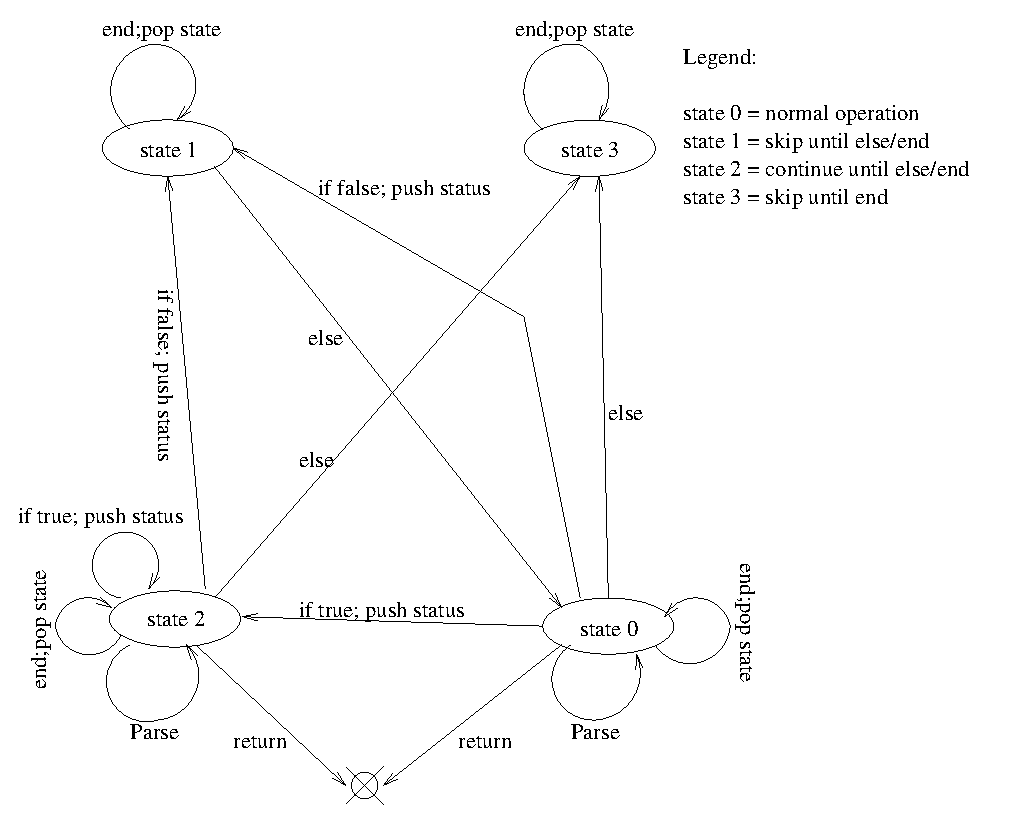
\includegraphics{parser_states.ps}}} \par}

\section{Logs, Error Codes and Debugging Info}
\subsection{Introduction}
The entire mud keeps all error codes and actions in a number of files in
great detail. These come in quite handy when debugging certain problems.
\paragraph{Error Codes}
\begin{itemize}
\item sql error codes
\item combat error codes
\item file io error codes
\end{itemize}

\paragraph{Log Files}
\begin{itemize}
\item error.txt, contains sql error codes
\item bigfile, contains all user input ever generated by all users
chronically
\item file error.log, contains all output from the combat system
\end{itemize}

\newpage
\section{Appendix A  - Table Description}

\subparagraph{action}table containing descriptions of special actions that
are allowed in some rooms
\subparagraph{answers}table containing all the different answers by bots on
questions asked
\subparagraph{bantable}table containing who is banned, why, by whom, for how
long at which time, etc.
\subparagraph{bogus\_itemtable}this is a very strange table that is currently being used as a temporary table for the cleaning up of corpses in the game. (see also the script
mysql\_healing)
\subparagraph{bottable}table containing the bots, gets copied periodically
to the tmp\_usertable by a crontab entry in order to add bots that people
have fought against and killed
\subparagraph{bugreportlist}list of bugs still to be solved
\subparagraph{containeditems}items that are not really active in the game
because they are currently 'trapped' so to speak inside containers (special
items that can contain items)
\subparagraph{depalias}special commands for the deputies to use
\subparagraph{help}help on commands
\subparagraph{items}item definitions
\subparagraph{itemtable}all items
\subparagraph{logonmessage}contains the logonmessage when you enter the game
\subparagraph{mailtable}all mail
\subparagraph{olditem}archived/deleted items
\subparagraph{oldmail}archived/deleted mail
\subparagraph{olduser}archived/deleted users
\subparagraph{respawningitemtable}items that need to reappear after a
certain time
\subparagraph{rooms}description of all rooms, along with exits
\subparagraph{sillynamestable}contains silly names/bad language in order to
root out bad logonids in entering the game
\subparagraph{skills}skill definitions
\subparagraph{skilltable}all skills
\subparagraph{tmp\_itemtable}items during gameplay
\subparagraph{tmp\_mailtable}mail during gameplay
\subparagraph{tmp\_usertable}users during gameplay
\subparagraph{todo}todo list
\subparagraph{unbantable}people that are allowed to login despite the fact
that their site/domain is banned
\subparagraph{usertable}all users
\subparagraph{commands}contains special commands
\subparagraph{methods}contains source code to perform by the mud
\subparagraph{events}contains events that run source code in the methods
table at specific times
\subparagraph{attributes}can contain 'special' attributes for characters,items,
rooms or even the game
\subparagraph{characterinfo}can contain extra information on characters for
generation of a charactersheet on the homepage.
\subparagraph{family}can contain family relations in addition to character
info for the charactersheet. See also characterinfo and familyvalues.
\subparagraph{familyvalues}contains a number of possible relations and their
corresponding unique id. See also 'family'.
\subparagraph{guilds}contains information regarding the guilds.

\newpage

\section{Appendix B  - Field Description}

\paragraph{usertable}
\subparagraph{name}the uniquely identifying name of a player character
\subparagraph{address}the ip address or host name from where the character
is being controlled
\subparagraph{password}the password of the person attempting to log on
\subparagraph{title}full title, can contain 254 characters
\subparagraph{realname}contains real name of player, field is optional
\subparagraph{email}contains email address of player, field is optional
\subparagraph{race}contains a race, there are a specific amount of races
available. They are: fox,
zombie, wyvern, wolf, turtle, troll, spider, slug, ropegnaw, rabbit, orc, ooze, human, elf, dwarf, duck, deity, chipmunk,
buggie. Currently the ones that are supported by the logon screen are Dwarf,
Human and Elf.
\subparagraph{sex}male or female
\subparagraph{age}description of age
\subparagraph{length}description
\subparagraph{width}description
\subparagraph{complexion}description
\subparagraph{eyes}description
\subparagraph{face}description
\subparagraph{hair}description
\subparagraph{beard}description
\subparagraph{arm}description
\subparagraph{leg}description
\subparagraph{gold}amount of gold coins person is carrying (default:0)
\subparagraph{silver}amount of silver coins person is carrying (default:0)
\subparagraph{copper}amount of copper coins person is carrying (default:2)
\subparagraph{room}roomnumber person is staying in at the moment (default:1)
\subparagraph{lok}used to store a 'SessionPassword', a password generated
upon logging in and used during gameplay.
\subparagraph{whimpy}contains the damage level at which a person will flee from a
fight. Depends on the current level of damage, and the maximum level of
damage necessary to kill the person. (default:0)
\subparagraph{experience}number providing experience points, 1000 points is
a level. So: 1324 would mean level 1, 324 experience points and 676 points
away from levelling to level 2. (default:0)
\subparagraph{fightingwho}name of person this person is fighing against
(attention, if this is person is actually fighting depends on a few factors
like 'is the enemy in the game', 'is the enemy in the same room', 'is the
enemy not asleep' etc) (default:'')
\subparagraph{sleep}1=asleep, 0=awake (default:0)
\subparagraph{punishment}number of ribbits away from normal self, should be
0
\subparagraph{fightable}1=cannot be fought by other person(only bot) 0=can
be fought by anyone (default:0)
\subparagraph{vitals}level of damage, see also maxvital (default:0)
\subparagraph{fysically}not used (default:0)
\subparagraph{mentally}not used (default:0)
\subparagraph{drinkstats}level of thirst (negative amounts=drunk) bigger
then 50 equals full of drink, smaller -59 equals full of alcohol  (default:0)
\subparagraph{eatstats}level of hunger <=50 otherwise full  (default:0)
\subparagraph{active}not used anymore  (default:0)
\subparagraph{lastlogin}last time command in game issued
\subparagraph{birth}first time logon
\subparagraph{god}god mode, 0=normal player, 1=god, 2=non-killable bot,
3=killable bot  (default:0)
\subparagraph{guild}description of guild, provides a means of ascertaining
wether or not person has a right to do certain guild commands (known guilds:
ds, knight, mif, rangers)  (default:'')
\subparagraph{strength}obvious?  (default:2)
\subparagraph{intelligence}obvious?  (default:2)
\subparagraph{dexterity}obvious?  (default:2)
\subparagraph{constitution}obvious?  (default:2)
\subparagraph{wisdom}obvious?  (default:2)
\subparagraph{practises}practise points to practise stuff like
fighting/swordplay/swimming/etc  (default:0)
\subparagraph{training}training points for upping the previous 5 stats
strength, intelligence, dexterity, constitution, wisdom (has immediate
influence on most skills)  (default:0)
\subparagraph{bandage}not used yet
\subparagraph{alignment}negative=bad, positive=good, 0=neutral, changes when
issueing fight  (default:0)
\subparagraph{manastats}magic stats  (default:0)
\subparagraph{movementstats}movements stats� (default:0)
\subparagraph{maxmana}maximum magic  (default:118)
\subparagraph{maxmove}maximum movement  (default:500)
\subparagraph{maxvital}maximum damage (death imminent)  (default:118)
\subparagraph{cgiServerSoftware}environment variables
\subparagraph{cgiServerName}environment variable
\subparagraph{cgiGatewayInterface}environment variable
\subparagraph{cgiServerProtocol}environment variable
\subparagraph{cgiServerPort}environment variable
\subparagraph{cgiRequestMethod}environment variable
\subparagraph{cgiPathInfo}environment variable
\subparagraph{cgiPathTranslated}environment variable
\subparagraph{cgiScriptName}environment variable
\subparagraph{cgiRemoteHost}environment variable
\subparagraph{cgiRemoteAddr}environment variable
\subparagraph{cgiAuthType}environment variable
\subparagraph{cgiRemoteUser}environment variable
\subparagraph{cgiRemoteIdent}environment variable
\subparagraph{cgiContentType}environment variable
\subparagraph{cgiAccept}environment variable
\subparagraph{cgiUserAgent}environment variable
\subparagraph{jumpmanaint}increase on magic when healing  (default:1)
\subparagraph{jumpmoveint}increase on movement when healing  (default:1)
\subparagraph{jumpvital}increase on damage when healing  (default:1)

\paragraph{skills}
\subparagraph{number}the id number of the skill (connection with skilltable
\subparagraph{name}the name of the skill, for example, \emph{Swordplay}
\subparagraph{inlevel}level needed at which the skill becomes available and can be learned
\subparagraph{outlevel}level at which the skill becomes to basic and is erased from memory
\subparagraph{manacost}the amount of mana it costs to use the skill or magic spell
\subparagraph{begineffect}description
\subparagraph{endeffect}description
\subparagraph{modifiername}1=Strength,2=Dexterity,3=Intelligence,4=Wisdom,
5=Constitution,...
\subparagraph{difficulty}1=easy,2=average,3=hard,4=veryhard
\subparagraph{type}1=normal skill, 2=fight skill, 3=magic skill, 4=cleric skill

\paragraph{skilltable}
\subparagraph{number}reference to skills-table
\subparagraph{forwhom}reference to tmpusertable/usertable
\subparagraph{skilllevel}

\paragraph{items}
\subparagraph{id}id number of the item
\subparagraph{name}noun
\subparagraph{adject1}first adjective
\subparagraph{adject2}second adjective
\subparagraph{adject3}third adjective (valid though never displayed)
\subparagraph{manaincrease}increases magic level by possession
\subparagraph{hitincrease}increases amount of damage done by fighting by
posession
\subparagraph{vitalincrease}increases damage resistance level by posession
(higher maxvital)
\subparagraph{movementincrease}increases the amount of movement possible
(higher maxmovement)
\subparagraph{eatable}description of what happens if the thing is eatable (if
description is empty, the object is not eatable)
\subparagraph{drinkable}description of what happens if the thing is drinkable (if
description is empty, the object is not drinkable)
\subparagraph{room}current room where the item resides (currently not used)
\subparagraph{lightable}not used
\subparagraph{getable}may be picked up
\subparagraph{dropable}may be dropped
\subparagraph{visible}is visible=1, is not visible=0
\subparagraph{wieldable}wether or not the item can be wielded in hand. 0=not
wieldable, 1=wieldable right hand, 2=wieldable left hand, 3=wieldable both
hands
\subparagraph{description}description of the item when looking upon it
\subparagraph{readdescr}description of item when attempting to read it (if
description is empty, the object is not readable)
\subparagraph{wearable}wether or not the item can be worn on body. 0=not
wearable, 1=wearable on lefthand, 2=wearable on right hand, 3=wearable on
both hands, 4=wearable on head, 7=wearable on neck, 8=wearable on head,
9=wearable on body, 10=wearable on legs, 11=wearable on feet
\subparagraph{gold}amount of gold coins the item costs
\subparagraph{silver}amount of silver coins the item costs
\subparagraph{copper}amount of copper coins the item costs
\subparagraph{weight}amount of weight in "units".
\subparagraph{pasdefense}amount of passive defense the item has when worn
\subparagraph{damageresistance}amount of damage it can deflect
\subparagraph{container}determines wether or not this item can act as a
repository for other items. If container equals 0, the item is not a
container/repository. Any other value will depict the number of weight units this
container can carry (although right now, this has not been implemented yet).

\paragraph{tmp\_itemtable}
This table, compared to the "itemtable" does not have any differences apart
from the fact that this table only contains the currently used items in the
game. The "itemtable" contains the items that are saved upon quitting the
game and are retrieved upon (re)entering the game.
\subparagraph{id}
id number of the item, foreign key to "items"
\subparagraph{search}where to search for the item, for example "rocks"
\subparagraph{belongsto}to whom the item(s) belongs (foreign key to name of
usertable)
\subparagraph{amount}number of items references here
\subparagraph{room}room number where the item is residing (0=not in a room,
belongs to someone)
\subparagraph{wearing}
where on body the item is worn. An empty string means that it isn't worn at
all. Possiblities are "lefthand", "righthand", "head", "neck", "head",
"body", "legs", "feet"
\subparagraph{wielding}
on which hand the item is wielded. An empty field meaning that it isn't
wielded at all. Possibilities are 1 (right hand) and 2 (left hand)
\subparagraph{containerid}
an identification of a container. If the field items.container is not equal
to 0, this item has the potential to be a container. If the containerid is
also not equal to 0, it means that this container contains items. The items
can be found by corroborating this containerid with the field
containeditems.containedin . One important message is that, if the
containerid has been set, the amount is automatically 1. 

\paragraph{containeditems}
This table is used to determine which items are contained in which
container.
\subparagraph{id}a unique number which identifies the definition of the
item. It must equal a unique number used in the items table.
\subparagraph{amount}the number/amount of this item available
\subparagraph{containedin}the container identification number. It maps to
the 'containerid' of the tmp\_itemtable and is the vital link into providing
which container is carrying which items inside.

\paragraph{commands}
This table is a part of the tables used by the parser. It can contain
special commands performed by users during gameplay.
\subparagraph{id}a unique number with which this command can be identified
\subparagraph{name}a unique name with which this command can be identified
\subparagraph{callable}an integer, if it is 0 the command has been disabled
\subparagraph{command}contains the command to be entered by the user to
activate the method, can contain wildcards
\subparagraph{method\_name}name of the method, points to the "methods" table
\subparagraph{args}currently not used, hope to have that changed soon.
\subparagraph{room}contains the room to be in if the command is to be
effective. When the room is 0, the command is available in every room.

\paragraph{methods}
\subparagraph{id}a unique number to identify the method
\subparagraph{name}a unique name to identify the method, is currently used
by the commands table
\subparagraph{src}the source code, this field can contain quite a bit of
text. See for examples the chapter "The Parser".

\paragraph{events}
\subparagraph{eventid}a unique number to identify the event
\subparagraph{name}a unique name to identify the event
\subparagraph{month}the month in which this event must be run. Allowed
values are 1-12. (if the field contains value -1, month is ignored)
\subparagraph{dayofmonth}the dayofmonth on which this event must be run. Allowed
values are 1-31. (if the field contains value -1, dayofmonth is ignored)
\subparagraph{hour}the hour in which this event must be run. Allowed
values are 0-23. (if the field contains value -1, hour is ignored)
\subparagraph{minute}the minute at which this event must be run. Allowed
values are 0-59. (if the field contains value -1, minute is ignored)
\subparagraph{dayofweek}the dayofweek on which this event must be run. Allowed
values are 1-7, where 1 equals Sunday. (if the field contains value -1, dayofweek is ignored)
\subparagraph{callable}an integer, if it is 0 the event has been disabled
\subparagraph{method\_name}name of the method, points to the "methods" table
\subparagraph{args}currently not used, hope to have that changed soon.
\subparagraph{room}contains the room number. 
When
the room is not 0, 'say'-command and 'sayeveryone'-command and all other 
output commands are directed to persons in that room.

\paragraph{attributes}
\subparagraph{name}a name for the attribute, it is perfectly possible to
have lots of the same names. To uniquely identify an attribute, use its
name,objectid and objecttype.
\subparagraph{value}the value of the attribute, this is a string by default,
however, the exact type is available in 'value\_type'
\subparagraph{value\_type}contains information on what kind of type the value
is. Possibilities are: string (simple text form) and integer (number form)
\subparagraph{objectid}contains uniquely identifying name for the object to
which an attribute belongs
\subparagraph{objecttype}contains the type of the object to which an
attribute belongs. 0=general game attribute, 1=character/user attribute,
2=room attribute, 3=item definition attribute, 4=iteminstance attribute

\paragraph{characterinfo}
\subparagraph{name}name of the character for which this record contains
info. Unique identifier.
\subparagraph{imageurl}url, link to image to be displayed on the
charactersheet.
\subparagraph{homepageurl}url, link to (owners) homepage
\subparagraph{dateofbirth}subjective, can be anything, but most normally a
written description of a date.
\subparagraph{cityofbirth}subjective, can be anything, from land to city to
shrubbery patch, but most normally the name of the city where born.
\subparagraph{storyline}large blob field, may contain the entire history of
the person/character in question. HTML tags are allowed.

\paragraph{family}
\subparagraph{name}name of character for which to specify family relations.
Currently the primary key is set to (name, toname). In case relations become
more complicated it is likely that that primary key need be expanded.
\subparagraph{toname}the name of the character to which the original
character has a relation.
\subparagraph{description}a number, refers to the table 'familyvalues' that
contains a description in text for each used number. For instance, daughter,
son, friend, etc.

\paragraph{familyvalues}
\subparagraph{id}unique identifying number for each type of relation.
\subparagraph{description}descriptive text of the relation, for example
daughter, son, friend, enemy, etc.

\paragraph{guilds}
\subparagraph{name}name of the guild. For example 'mif' or 'rangers'.
\subparagraph{title}full title of the guild.
\subparagraph{description}description of what the guild is for/does exactly.
\subparagraph{location}where the guild can be found in the game.
\subparagraph{homepage}where the homepage of the guild can be found on the
web.
\subparagraph{leader}name of the character currently in control as the
'guildmaster'.

\newpage

\section{Appendix C - Database Structure}

{\par\centering
\resizebox*{1\textwidth}{!}{\rotatebox{0}{\includegraphics{database.ps}}} \par}

\newpage

\section{Appendix D - Rolls Analysis}

First "main" started.

"main" starts "StartSQL".

"StartSQL" uses "checkBestHand" to determine which hand (along with which
item) to use during combat, so, depending on outcome of "checkBestHand"
"StartSQL" determines wether to choose "right" or "left". Two choices in the
If-then statement.

"checkBestHand" provides you with wether the "right" hand or the "left" hand
is the best. There are three possible scenarios, neither hand contains an
item (returns right hand), one hand contains item (returns hand that
contains item) and both hands contain items (returns hand with best shot).
In the last case, "checkBestHand" uses "checkWeaponSkill" to determine which
one of the two hands has the better skill in item carrying.

After that, the "AttackRoll" determines wether or not the attempt to strike
your opponent is successfull. Either it is successfull (you hit your
opponent) or it isn't successfull (you missed). However, there is the
possiblity of a FANTASTIC success or a FATAL failure, which is just an
extreme version of the previously described process.

After the Attackroll has been successfull, it is necessary to compute a
"DefenseRoll". If the defense of your opponent is successfull, you succeed
in hitting him but do not do any damage. 

If your opponent fails to defend himself, you have to have a "DamageRoll".
The DamageRoll determines how much of your hit has been transferred to
actual damagepoints on the part of your opponent.

{\par\centering
\resizebox*{1\textwidth}{!}{\rotatebox{270}{\includegraphics{rolls2.ps}}} \par}

\newpage
\section{Appendix E - Examples of Skills}

Unarmed Combat
\newline
Dodge
\newline
Parry (with most weapons)
\newline
Block (only with shield)
\newline
Combat Reflexes
\newline
Thrusting
\newline
Swinging
\newline
Throwing
\newline
Impaling

\newpage
\section{Appendix F - Links to Visit}

\subparagraph{www.karchan.org}
\subparagraph{www.linux.org}
\subparagraph{www.ssh.org}
\subparagraph{www.mysql.com}
\subparagraph{www.boutell.com}
\subparagraph{www.gnu.org}
\subparagraph{www.apache.org}
\subparagraph{www.cvshome.org}

\newpage
\section{Appendix G - Glossary}

\subparagraph{apache}software that runs a web server for you. If you don't
know what a web server is, you probably shouldn't be reading this document.

\subparagraph{C}If not THE programming language, it is a programming
langugage. Definitions are abound, look them up.

\subparagraph{CGI}Some people claim is means Computer Generate Images. But
in this document's context it stands for Common Gateway Interface, and is
one of the few standard ways with which a Web Browser is able to transmit
data entered by the user to a script/program/application residing on a server.
If you've ever visited a search engine, you've used it.
The mud is built on this principle. (See www.boutell.com)

\subparagraph{cookie}A cookie is an extension to the HTTP protocol, to allow
small amounts of information to be saved on the client computer that
accesses a web server. This without jeopardizing security. The browser itself
is responsible for honoring/denying cookies. Cookies contain a name, a
value, a hostname from which they originated, and a path from which the page
was sent that contained the cookie as well as an expiration date. Only the
name and value are obligatory. See the part on password authorisation.

\subparagraph{copyleft}The opposite of copyright in some ways. See GPL.

\subparagraph{crontab}a Unix tool that starts programs/scripts/applications
at specific recurring times without user interference.

\subparagraph{CVS}Concurrent Version System, used in order to keep tabs on
changes on the source code of the mud by using Version Control.

\subparagraph{database}information storage and retrieval. Information is
stored within tables inside the database.

\subparagraph{field}a database object, is contained in a record, has a
possible value.

\subparagraph{foreign key}a database object, an index on a table referring
to another table. Currently the database in use, MySQL, does not contain
physical foreign keys. But is also denotes logical foreign keys. A foreign
key in one table refers to a primary key in another table. For example that
a record in the itemtable contains a foreign key to the primary key (name)
of the user table.

\subparagraph{FSF}Free Software Foundation, a foundation established by
Richard M. Stallman, who devoted his life in the quest to make all software
freely available (free as in speech, not beer). Lots of tools fall under the
FSF of which this mud uses plenty. See GPL.

\subparagraph{GNU}GNU's Not Unix, yes that's right, it is a recursive
abbreviation/acronym. You see these alot in Unix/Linux environments. It is also
called the FSF. I suggest you look there.

\subparagraph{GPL}Gnu's General Public License, it is a copyright notice that lets
people copy and distribute and change the source code provided under this
copyright. It also means that you are not allowed NOT to deliver the source
code along with any distribution you might make. This in order to protect
the fact that software should always be free. GPL originally designed and
set up by GNU. See GNU.

\subparagraph{HTTP}Hyper Text Transfer Protocol, protocol used for
communication between Web Browsers and Web Servers.

\subparagraph{husking}idling, not doing anything because you are busy doing
something else. Also known as AFK (Away From Keyboard).

\subparagraph{Linux}A Unix-like Operating System developed by Linus
Thorvals, with tools by Richard M. Stallman of GNU.

\subparagraph{MUD}MUD, from the Hackers' Dictionary:
MUD: /muhd/ [acronym, Multi-User Dungeon; alt. Multi-User
Dimension] 1. n.  A class of {virtual reality} experiments
accessible via the Internet.  These are real-time chat forums with
structure; they have multiple 'locations' like an adventure game, 
and may include combat, traps, puzzles, magic, a simple economic  
system, and the capability for characters to build more structure 
onto the database that represents the existing world.  2. vi. To  
play a MUD (see {hack-and-slay}).  The acronym MUD is often
lowercased andor verbed; thus, one may speak of 'going
mudding', etc.

Historically, MUDs (and their more recent progeny with names of MU-
form) derive from an AI experiment by Richard Bartle and Roy
Trubshaw on the University of Essex's DEC-10 in the early 1980s;
descendants of that game still exist today (see {BartleMUD}).   
The title 'MUD' is still trademarked to the commercial MUD run by
Bartle on British Telecom (the motto: "You haven't *lived*
'til you've *died* on MUD!"); however, this did not stop  
students on the European academic networks from copying and improving
on the MUD concept, from which sprung several new MUDs (VAXMUD,
AberMUD, LPMUD).  Many of these had associated bulletin-board  
systems for social interaction.  Because USENET feeds have been
spotty and difficult to get in the U.K.  and the British JANET 
network doesn't support {FTP} or remote login via telnet, the  
MUDs became major foci of hackish social interaction there.    

AberMUD and other variants crossed the Atlantic around 1988 and
quickly gained popularity in the U.S.; they became nuclei for large
hacker communities with only loose ties to traditional hackerdom   
(some observers see parallels with the growth of USENET in the     
early 1980s).  The second wave of MUDs (TinyMUD and variants)      
tended to emphasize social interaction, puzzles, and cooperative   
world-building as opposed to combat and competition.  In 1991, over
50\% of MUD sites are of a third major variety, LPMUD, which
synthesizes the combat/puzzle aspects of AberMUD and older systems
with the extensibility of TinyMud. The trend toward greater
programmability and flexibility will doubtless continue.   

The state of the art in MUD design is still moving very rapidly,
with new simulation designs appearing (seemingly) every month.  
There is now (early 1991) a move afoot to deprecate the term    
{MUD} itself, as newer designs exhibit an exploding variety of  
names corresponding to the different simulation styles being    
explored. 

\subparagraph{MYSQL}a database, originally designed by TcX Consulting as I
recall. See 'database'.

\subparagraph{NULL}a database value representing an field that has not been
filled out, or in programming a pointer pointing to nothing.

\subparagraph{primary key}a database object, an index on a table uniquely
identifying each record by one or a combination of fields. See also foreign
key.

\subparagraph{record}a database object, containing fields. A table contains
a number of records.

\subparagraph{SQL}Standard Query Language. Simple 'programming' language
used to interface with a database for information mutation and retrieval.

\subparagraph{SSH}Secure Shell, it is an encrypted replacement of Telnet and
therefore more secure.

\subparagraph{table}a database object, containing records. Each record in a
table can be identified by its primary key.

\subparagraph{Telnet}A protocol or program to connect to a remote computer,
called a server, for remote administration/management. See also Secure Shell,
for it's more robust counterpart

... your text goes here ...
\end{document}
